\documentclass[11pt,a4paper]{article}
%%%----------------------------------------------------------------------------%%%
%%%----------------------------------------------------------------------------%%%
%%% 
%%% ### Packages 
%%%
%%%----------------------------------------------------------------------------%%%
%%%----------------------------------------------------------------------------%%%
\usepackage{amsmath, amsthm, amssymb, nccbbb, bm, dsfont, pifont, fontawesome, graphicx, varioref, enumitem, mathtools, listings, xcolor, cite, fancyhdr, lastpage, lscape, subfig, graphicx, float, tabularx, algpseudocode, algorithm}

\RequirePackage[round,authoryear]{natbib}
\RequirePackage[colorlinks,citecolor=blue,urlcolor=blue]{hyperref}
\usepackage[cal=boondox]{mathalfa}
%\usepackage[numbers]{natbib}
\setlength{\topmargin}{-0.5in}
\setlength{\textheight}{10in}
\setlength{\oddsidemargin}{-.6in}
\setlength{\textwidth}{7.5in}
\hypersetup{colorlinks=true, linkcolor=blue, citecolor=red, urlcolor=blue}

%%%----------------------------------------------------------------------------%%%
%%%----------------------------------------------------------------------------%%%
%%% 
%%% ### Code 
%%%
%%%----------------------------------------------------------------------------%%%
%%%----------------------------------------------------------------------------%%%
\usepackage{listings}
\lstset{escapeinside=| |}
\usepackage[usenames,dvipsnames]{color}  
\definecolor{mygray}{rgb}{0.99,0.99,0.99}
\definecolor{myblue}{rgb}{0.0, 0.23, 0.63}
\definecolor{myred}{rgb}{0.75, 0.0, 0.0}
\definecolor{mygreen}{rgb}{0.4, 0.69, 0.2}  
\lstnewenvironment{R}{\lstset{ 
  language=R,
  basicstyle=\footnotesize\ttfamily, 
  numbers=left,
  numberstyle=\tiny\color{black},
  stepnumber=1,
  numbersep=5pt,
  backgroundcolor=\color{mygray},
  showspaces=false, 
  showstringspaces=false,
  showtabs=false, 
  frame=single,  
  rulecolor=\color{black},
  tabsize=4,
  captionpos=b,
  breaklines=true,
  breakatwhitespace=false,
  keywordstyle=\ttfamily\bfseries\color{myblue},
  commentstyle=\ttfamily\bfseries\color{myred},
  stringstyle=\ttfamily\bfseries\color{mygreen}
} 
}{}

%New colors defined below
\definecolor{codegreen}{rgb}{0,0.6,0}
\definecolor{codegray}{rgb}{0.5,0.5,0.5}
\definecolor{codepurple}{rgb}{0.58,0,0.82}
\definecolor{backcolour}{rgb}{0.95,0.95,0.92}

%Code listing style named "mystyle"
\lstdefinestyle{mystyle}{
  backgroundcolor=\color{backcolour}, commentstyle=\color{codegreen},
  keywordstyle=\color{magenta},
  numberstyle=\tiny\color{codegray},
  stringstyle=\color{codepurple},
  basicstyle=\ttfamily\footnotesize,
  breakatwhitespace=false,         
  breaklines=true,                 
  captionpos=b,                    
  keepspaces=true,                 
  numbers=left,                    
  numbersep=5pt,                  
  showspaces=false,                
  showstringspaces=false,
  showtabs=false,                  
  tabsize=2
}

%"mystyle" code listing set
\lstset{style=mystyle}

%%%----------------------------------------------------------------------------%%%
%%%----------------------------------------------------------------------------%%%
%%% 
%%% ### Box
%%%
%%%----------------------------------------------------------------------------%%%
%%%----------------------------------------------------------------------------%%%
\usepackage{tcolorbox}
\tcbuselibrary{breakable}
\newtcolorbox{mybox}{colback=yellow!5!white, colframe=gray!60!black, breakable}
\newtcolorbox{mybox0}{colback=white, colframe=gray!60!black, breakable}
	

%%%----------------------------------------------------------------------------%%%
%%%----------------------------------------------------------------------------%%%
%%% 
%%% ### Theorem style structures 
%%%
%%%----------------------------------------------------------------------------%%%
%%%----------------------------------------------------------------------------%%%
\numberwithin{equation}{section}
\theoremstyle{plain}
\newtheorem{theorem}{Theorem}[section]
\newtheorem{lemma}[theorem]{Lemma}
\newtheorem{corollary}[theorem]{Corollary}
\newtheorem{proposition}[theorem]{Proposition}
\newtheorem{condition}{Condition}[section]
\newtheorem{definition}{Definition}[section]
\theoremstyle{definition}
\newtheorem{example}{Example}[section]
\newtheorem{exercise}{Exercise}[section]
\newtheorem{remark}{Remark}[section]
\newtheorem{remark0}{Remark}
\newtheorem{question}{Question}


%%%----------------------------------------------------------------------------%%%
%%%----------------------------------------------------------------------------%%%
%%% 
%%% ### Operators 
%%%
%%%----------------------------------------------------------------------------%%%
%%%----------------------------------------------------------------------------%%%
\newcommand{\pr}{\mathsf{P}} 
\newcommand{\E}{\mathsf{E}} 
\newcommand{\median}{\mathop{\mathsf{median}}}
\newcommand{\Cov}{{\mathsf{Cov}}} 
\newcommand{\Corr}{{\mathsf{Corr}}} 
\newcommand{\Var}{{\mathsf{Var}}}
\newcommand{\SD}{{\mathsf{SD}}}
\newcommand{\CV}{{\mathsf{CV}}}
\newcommand{\Bias}{{\mathsf{Bias}}}
\newcommand{\AMSE}{\operatorname{\mathsf{AMSE}}}
\newcommand{\MSE}{\operatorname{\mathsf{MSE}}}
\newcommand{\ARE}{\mathsf{ARE}}
\newcommand{\AV}{\mathsf{AV}}
\newcommand{\CRLB}{{\mathsf{CRLB}}}

\newcommand{\pCorr}{\text{P}}
\newcommand{\sCorr}{\text{S}}
\newcommand{\kCorr}{\text{K}}
\newcommand{\bdCorr}{\text{BD}}
\newcommand{\cCorr}{\text{C}}


\newcommand{\inD}{    \overset{ \textnormal{d}   }{\rightarrow} }
\newcommand{\inAS}{   \overset{ \textnormal{a.s.}   }{\rightarrow} }
\newcommand{\inP}{    \overset{ \textnormal{pr}    }{\rightarrow} }
\newcommand{\inLp}{   \overset{ \mathcal{L}^p }{\rightarrow} }
\newcommand{\inMSE}{  \overset{ \textnormal{qm} }{\rightarrow} }
\newcommand{\inQM}{   \overset{ \textnormal{qm} }{\rightarrow} }
\newcommand{\indep}{\protect\mathpalette{\protect\independenT}{\perp}}
\def\independenT#1#2{\mathrel{\rlap{$#1#2$}\mkern4mu{#1#2}}}
\newcommand{\iid}{\textsc{iid}} 
\newcommand{\simIID}{   \overset{ \iid   }{\sim} }
\newcommand{\simIND}{   \overset{ {\indep}   }{\sim} }


\newcommand{\Bern}{\textnormal{Bern}} 
\newcommand{\Unif}{\textnormal{Unif}} 
\newcommand{\Normal}{\textnormal{N}} 
\newcommand{\logNormal}{\textnormal{LN}} 
\newcommand{\Bin}{\textnormal{Bin}} 
\newcommand{\NB}{\textnormal{NB}} 
\newcommand{\HG}{\textnormal{HG}} 
\newcommand{\Geom}{\textnormal{Geom}} 
\newcommand{\Beta }{\textnormal{Beta}} 
\newcommand{\BetaBin}{\textnormal{Beta-Bin}}
\newcommand{\Ga}{\textnormal{Ga}} 
\newcommand{\Exp}{\textnormal{Exp}} 
\newcommand{\Expo}{\textnormal{Expo}} 
\newcommand{\Po}{\textnormal{Po}} 
\newcommand{\Multi}{\textnormal{Multi}} 
\newcommand{\student}{\textnormal{t}} 
\newcommand{\Cauchy}{\textnormal{Cauchy}} 
\newcommand{\Pareto}{\textnormal{Pareto}} 
\newcommand{\Laplace}{\textnormal{Laplace}} 
\newcommand{\Logistic}{\textnormal{Logistic}} 
\newcommand{\Dir}{\textnormal{Dir}} 
\newcommand{\DP}{\textnormal{DP}} 
\newcommand{\Inv}{\textnormal{Inv-}} 
\newcommand{\F}{\textnormal{F}} 
\newcommand{\sign}{\textnormal{sign}}
\newcommand{\rank}{\textnormal{rank}}


\newcommand{\RV}{\textsc{rv}}
\newcommand{\cdf}{\textsc{cdf}} 
\newcommand{\cgf}{\textsc{cgf}} 
\newcommand{\pdf}{\textsc{pdf}} 
\newcommand{\pmf}{\textsc{pmf}} 
\newcommand{\chf}{\textsc{chf}} 
\newcommand{\mgf}{\textsc{mgf}}
\newcommand{\EF}{\textsc{EF}}
\newcommand{\NEF}{\textsc{NEF}}
\newcommand{\MLE}{\textsc{mle}}
\newcommand{\MAP}{\textsc{MAP}}
\newcommand{\Med}{\textsc{Med}}
\newcommand{\MME}{\textsc{mme}}
\newcommand{\QME}{\textsc{qme}}
\newcommand{\UMVUE}{\textsc{umvue}}
\newcommand{\MPT}{\textsc{MPT}}
\newcommand{\UMPT}{\textsc{UMPT}}
\newcommand{\LRT}{\textsc{LRT}}


\newcommand{\diag}{\mathop{\mathrm{diag}}}
\newcommand{\tr}{\mathop{\mathrm{tr}}}
\newcommand{\T}{\mathop{\mathrm{T}}}
\DeclareMathOperator*{\argmin}{arg\,min}
\DeclareMathOperator*{\argmax}{arg\,max}
\DeclareMathOperator{\sgn}{sgn}
\DeclareMathOperator{\logit}{logit}
\DeclareMathOperator{\expit}{expit}
\newcommand{\dd}{\textnormal{d}}


\newcommand{\lva}{{\color{myred}\ding{73}\ding{73}\ding{73}}}
\newcommand{\lvb}{{\color{myred}\ding{72}\ding{73}\ding{73}}}
\newcommand{\lvc}{{\color{myred}\ding{72}\ding{72}\ding{73}}}
\newcommand{\lvd}{{\color{myred}\ding{72}\ding{72}\ding{72}}}
\newcommand{\optional}{\noindent{\color{myblue}\faScissors}}
\newcommand{\Solution}{\noindent{\color{myblue}{{\textsc{Solution}}:~$\Big.$}}}
\newcommand{\take}{\noindent{\color{myblue}\faPaperPlaneO~\underline{\bf Takeaway}:~$\Big.$}}

% widecheck 
\DeclareFontFamily{U}{mathx}{\hyphenchar\font45}
\DeclareFontShape{U}{mathx}{m}{n}{
      <5> <6> <7> <8> <9> <10>
      <10.95> <12> <14.4> <17.28> <20.74> <24.88>
      mathx10
      }{}
\DeclareSymbolFont{mathx}{U}{mathx}{m}{n}
\DeclareFontSubstitution{U}{mathx}{m}{n}
\DeclareMathAccent{\widecheck}{0}{mathx}{"71}
\DeclareMathAccent{\wideparen}{0}{mathx}{"75}

\def\cs#1{\texttt{\char`\\#1}}

% Customize header and footer
\pagestyle{fancy}
\fancyhf{}
\fancyhead[L]{2021-22 Semester 2}
\fancyhead[R]{STAT4012 Statistical Principles of Deep Learning with Business}
\fancyfoot[R]{Page \thepage\ of \pageref*{LastPage}}
\fancyfoot[L]{\nouppercase{\leftmark}}
\renewcommand{\headrulewidth}{0.4pt} % default is 0pt
\renewcommand{\footrulewidth}{0.4pt} % default is 0pt

\usepackage[bottom]{footmisc}

\newcounter{magicrownumbers}
\newcommand\rownumber{\stepcounter{magicrownumbers}\arabic{magicrownumbers}}

\usepackage[table]{xcolor}
%------------------------------------------------------------------------------

\begin{document}
    
    % Page 0 for names and table of contents
    \thispagestyle{empty}
    \pagenumbering{gobble} 
    \title{\textsc{STAT 4012} -- Statistical Principles of Deep Learning with Business \\ Group Project}
    \author{
        KWOK Ho Hin (SID: \texttt{1155126159}) \\
        LAI Tsz Chun (SID: \texttt{1155125208}) \\
        LAM Wai Chui (SID: \texttt{1155152095}) \\
        LAW Yiu Leung Eric (SID: \texttt{1155149315}) \\
        TSOI Tung Sing (SID: \texttt{1155127274}) \\
        LO Chak Kin Steven (SID: \texttt{1155125491})
    }
    \date{\today}
    \maketitle
    
    % \newpage
    \tableofcontents
    \thispagestyle{empty}
    \pagenumbering{gobble} 
    \newpage
    
    % Section 1
    \pagenumbering{arabic}
    \setcounter{page}{1}
    
    % Emotion Detection
    \section{Real Time Emotion Detection Deep Learning Model}
    \textbf{This section is contributed by LAI Tsz Chun (SID: 1155125208), LAM Wai Chui (SID: 1155152095) and LAW Yiu Leung Eric (SID: 1155149315).}
    
    \subsection{Introduction}
    This is an introduction.
    
    \subsection{Dataset}
    \href{https://www.kaggle.com/datasets/msambare/fer2013}{FER-2013} \cite{FER2013} dataset from Kaggle is selected for model training. The data consists of 48x48 pixel grayscale images of faces. The faces have been automatically registered so that the face is more or less centred and occupies about the same amount of space in each image. The faces are categorized into seven categories (0=Angry, 1=Disgust, 2=Fear, 3=Happy, 4=Neutral, 5=Sad, 6=Surprise). The training set consists of 28,709 examples and the public test set consists of 3,589 examples. 
    \begin{figure}[H]
        \centering
        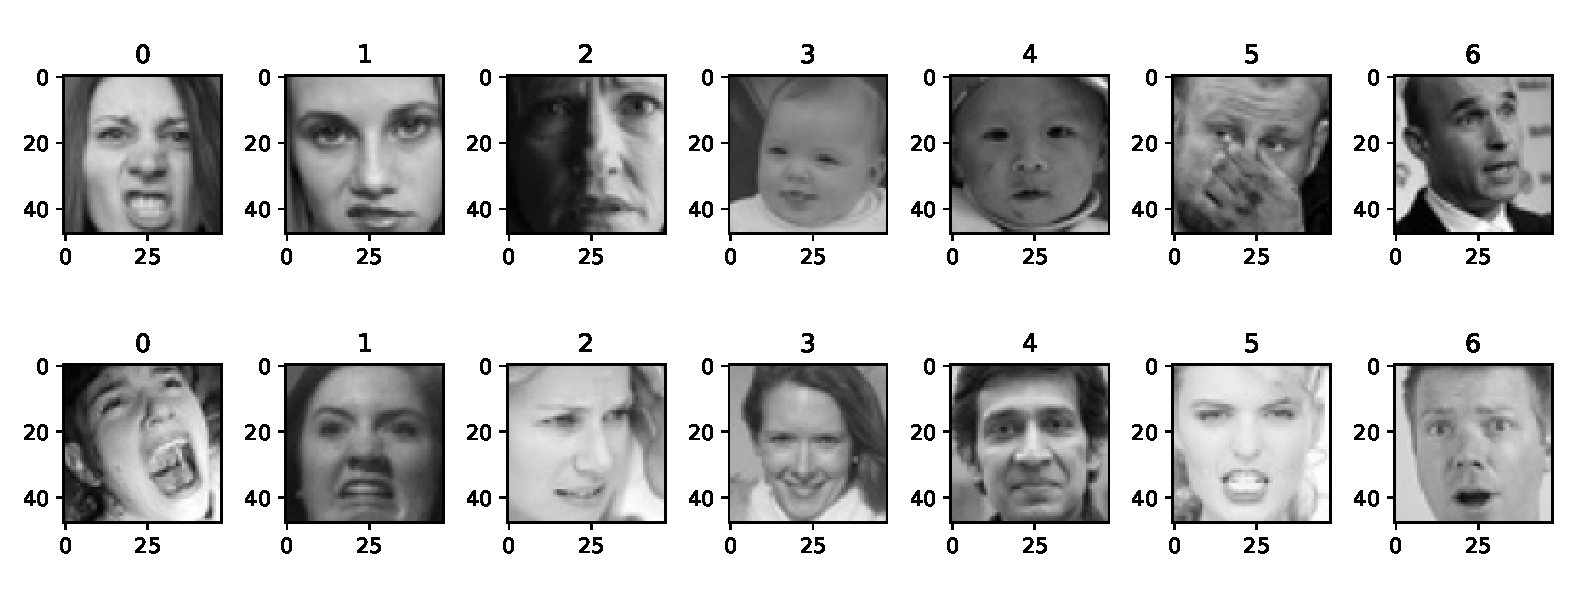
\includegraphics[width = 0.9\textwidth]{emotion_detection/plot/train.pdf}
        \caption{Training Dataset}
        \label{fig:train_dataset}
    \end{figure}
    \begin{figure}[H]
        \centering
        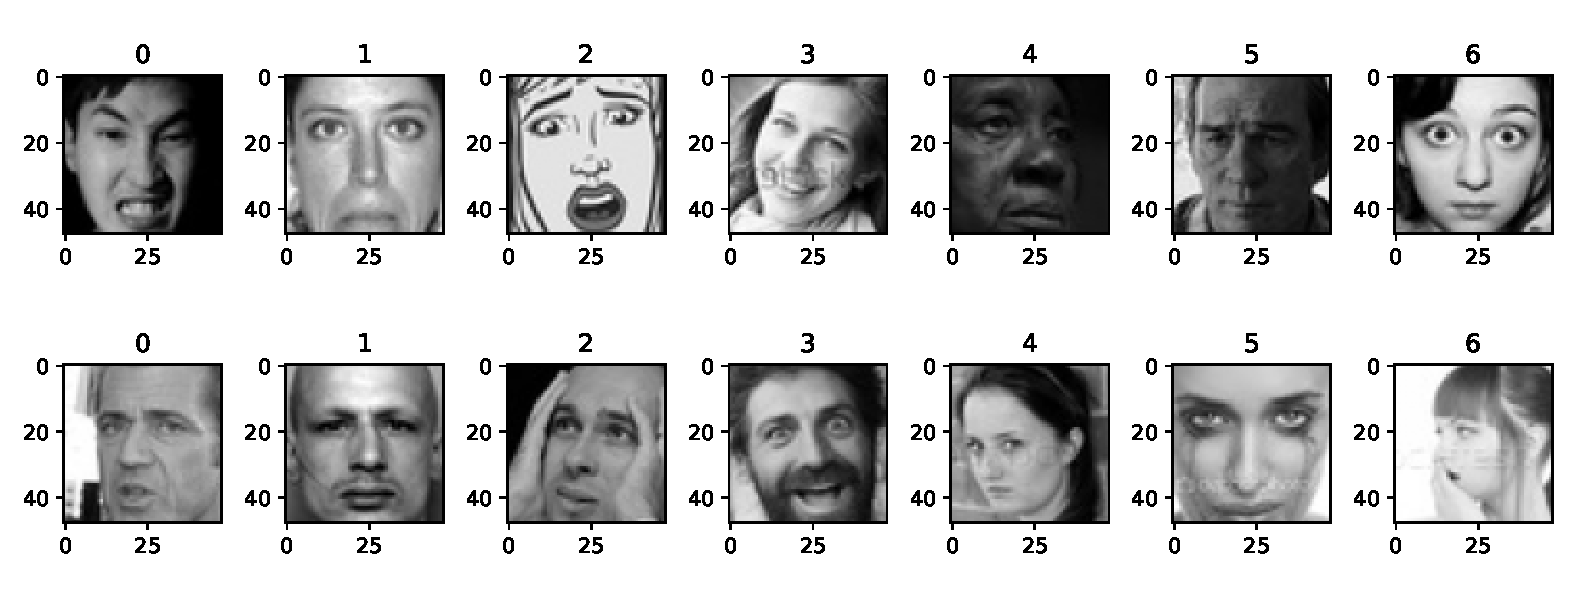
\includegraphics[width = 0.9\textwidth]{emotion_detection/plot/test.pdf}
        \caption{Testing Dataset}
        \label{fig:test_dataset}
    \end{figure}
    
    % \subsection{Project Description}
    
    \subsection{Data Preparation for Model Training}
    The data are stored in \texttt{.jpg} format, in order to use them, we must perform pre-processing to the dataset.
    \begin{enumerate}
        \item Read the images using \texttt{OpenCV}.
        \item Normalized the grayscale from [0, 255] to [0, 1] for increasing training speed.
        \item Stack up 1-channel grayscale array into 3-channel RGB array, as the final use would be RGB pictures.
        \item Encode the labels.
        \item Save the array to \texttt{NumPy} array, then save as \texttt{Pickle} file.
    \end{enumerate}
    Noted that the dataset have already split into training and testing datasets from Kaggle, we do not need to split them. \\
    \textbf{Implementation:} \texttt{emotion\_detection\textbackslash src\textbackslash read\_data.ipynb}
        
    % \subsubsection{Create Numpy Array}
    
    % \subsubsection{Splitting Training Dataset and Testing Dataset}
    
    \subsection{Model Design}
    We intended to build a real-time emotion detection AI, so there are two separated models needed, namely face detection model and emotion detection model. Flow of the model:
    \begin{enumerate}
        \item Detect face(s) in a photo.
        \item Capture pixels of the face(s) and resize to 48x48.
        \item Classify emotion of the faces(s).
    \end{enumerate}
    
    \subsubsection{MTCNN Face Detection Model}
    MTCNN is a python (pip) library written by Github user \href{https://github.com/ipazc/mtcnn}{ipacz} \cite{MTCNN}, which implements the paper by Zhang, Kaipeng et al. “Joint Face Detection and Alignment Using Multitask Cascaded Convolutional Networks.” \cite{1604.02878} In this paper, they propose a deep cascaded multi-task framework using different features of “sub-models” to each boost their correlating strengths. We choose MTCNN model for detecting faces in picture.
    \begin{figure}[H]
        \centering
        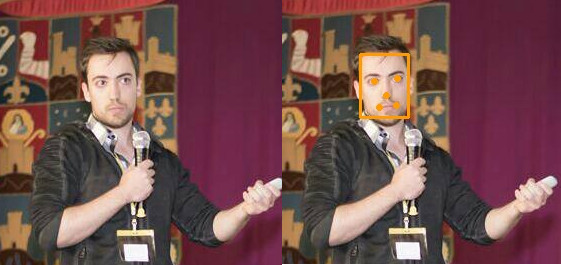
\includegraphics[width = 0.8\textwidth]{written_report/pictures/mtcnn.jpg}
        \caption{Face Detection using MTCNN}
        \label{fig:MTCNN}
    \end{figure}
    
    \subsubsection{Augmentation}
    
    
    \subsubsection{Emotion Detection Model}
    We create and train a custom CNN model, which includes 5 blocks of convolution layers and 2 hidden fully-connected layers. All convolution layers and hidden layers  are using RELU activation, expect the output layer is using softmax activation.
    \begin{figure}[H]
        \centering
        \begin{minipage}[b]{.4\textwidth}
            \centering
            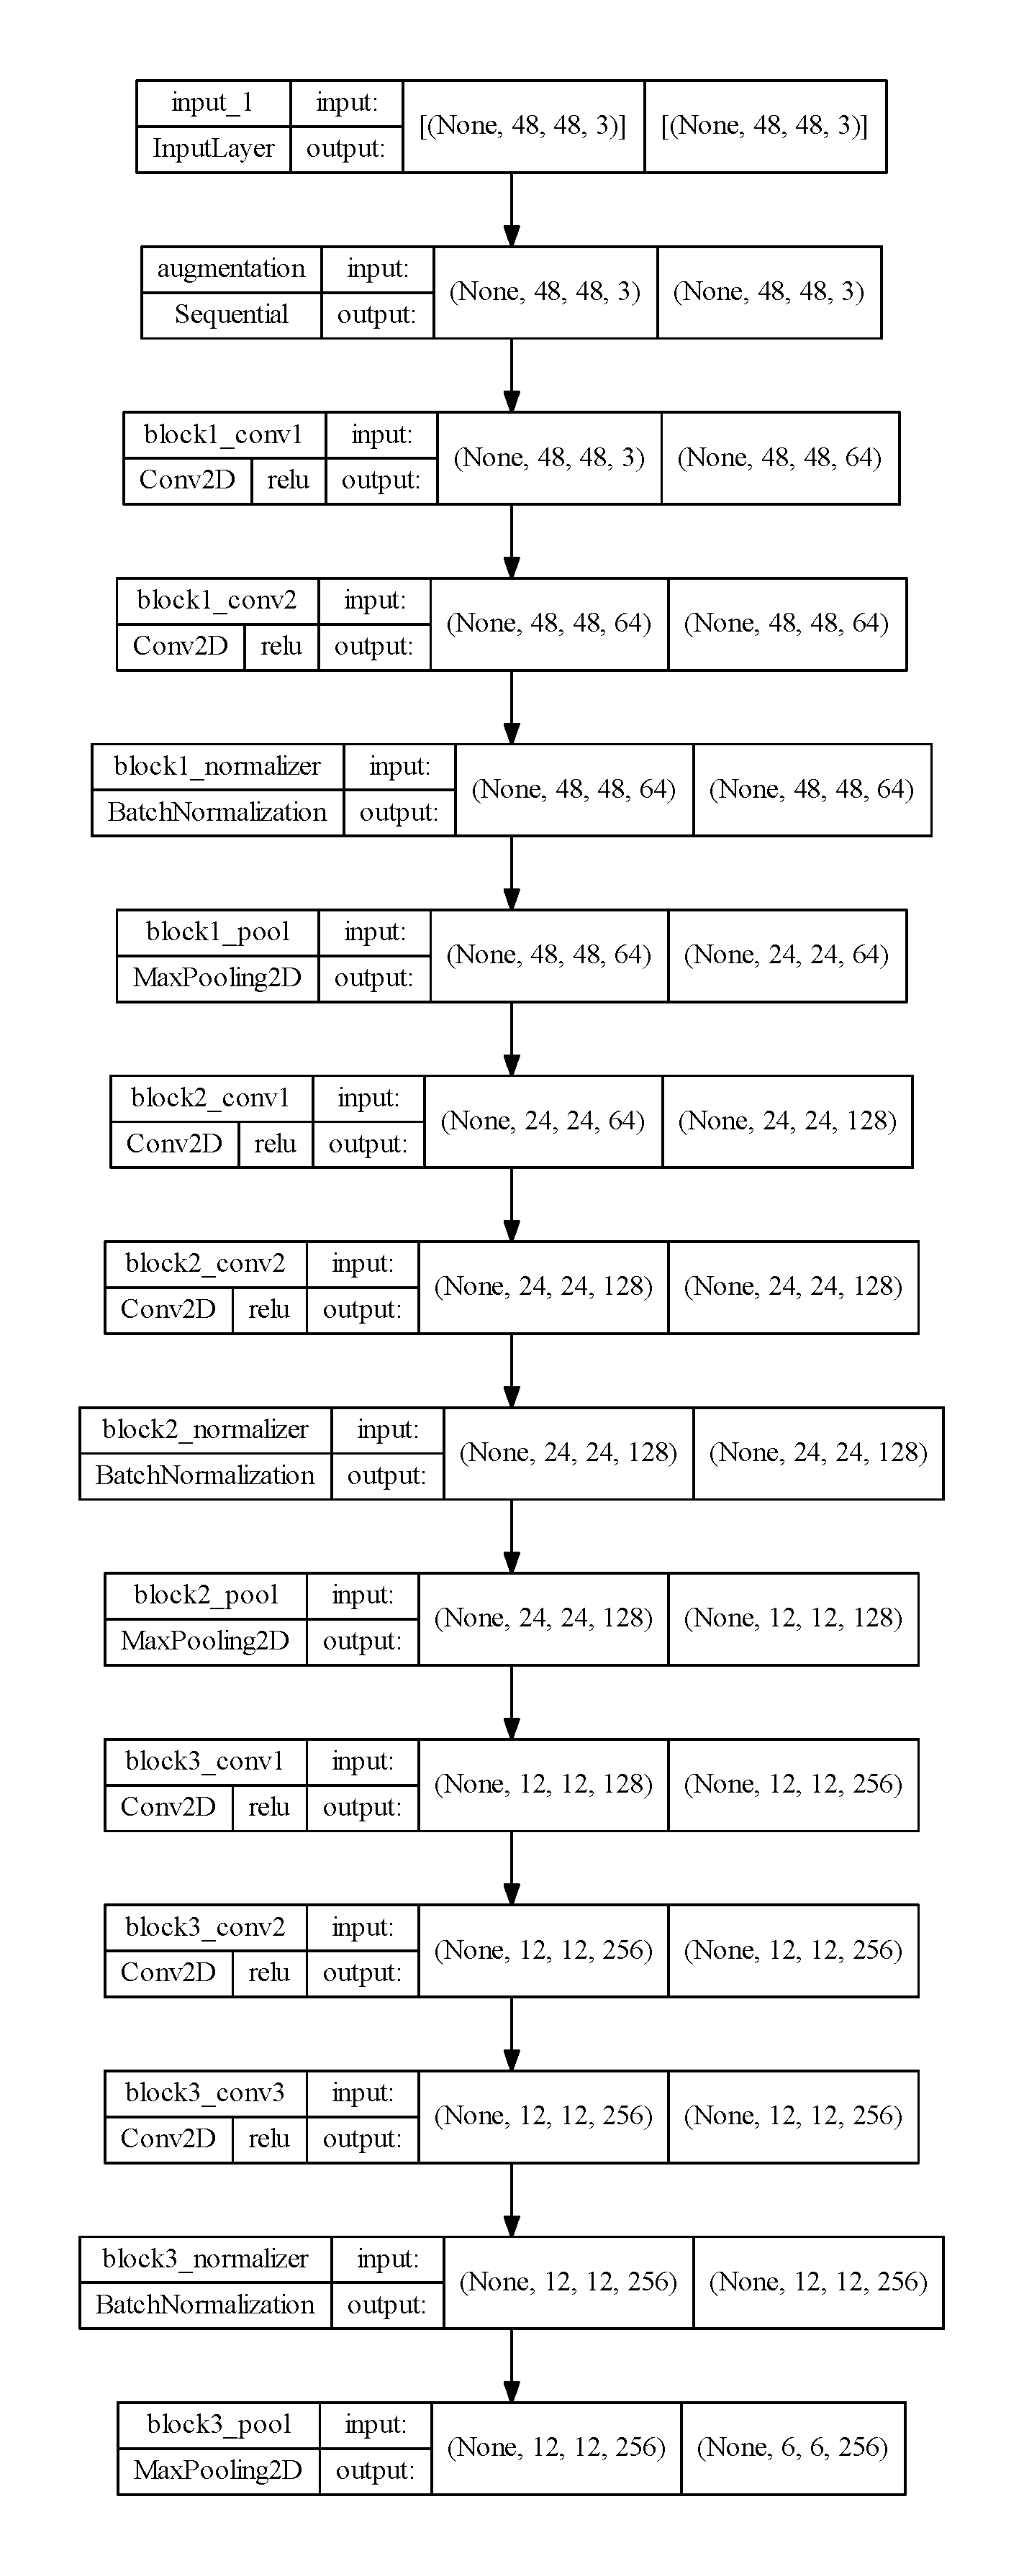
\includegraphics[height = 0.9\textheight]{written_report/pictures/model_1.pdf}
        \end{minipage}
        \begin{minipage}[b]{.4\textwidth}
            \centering
            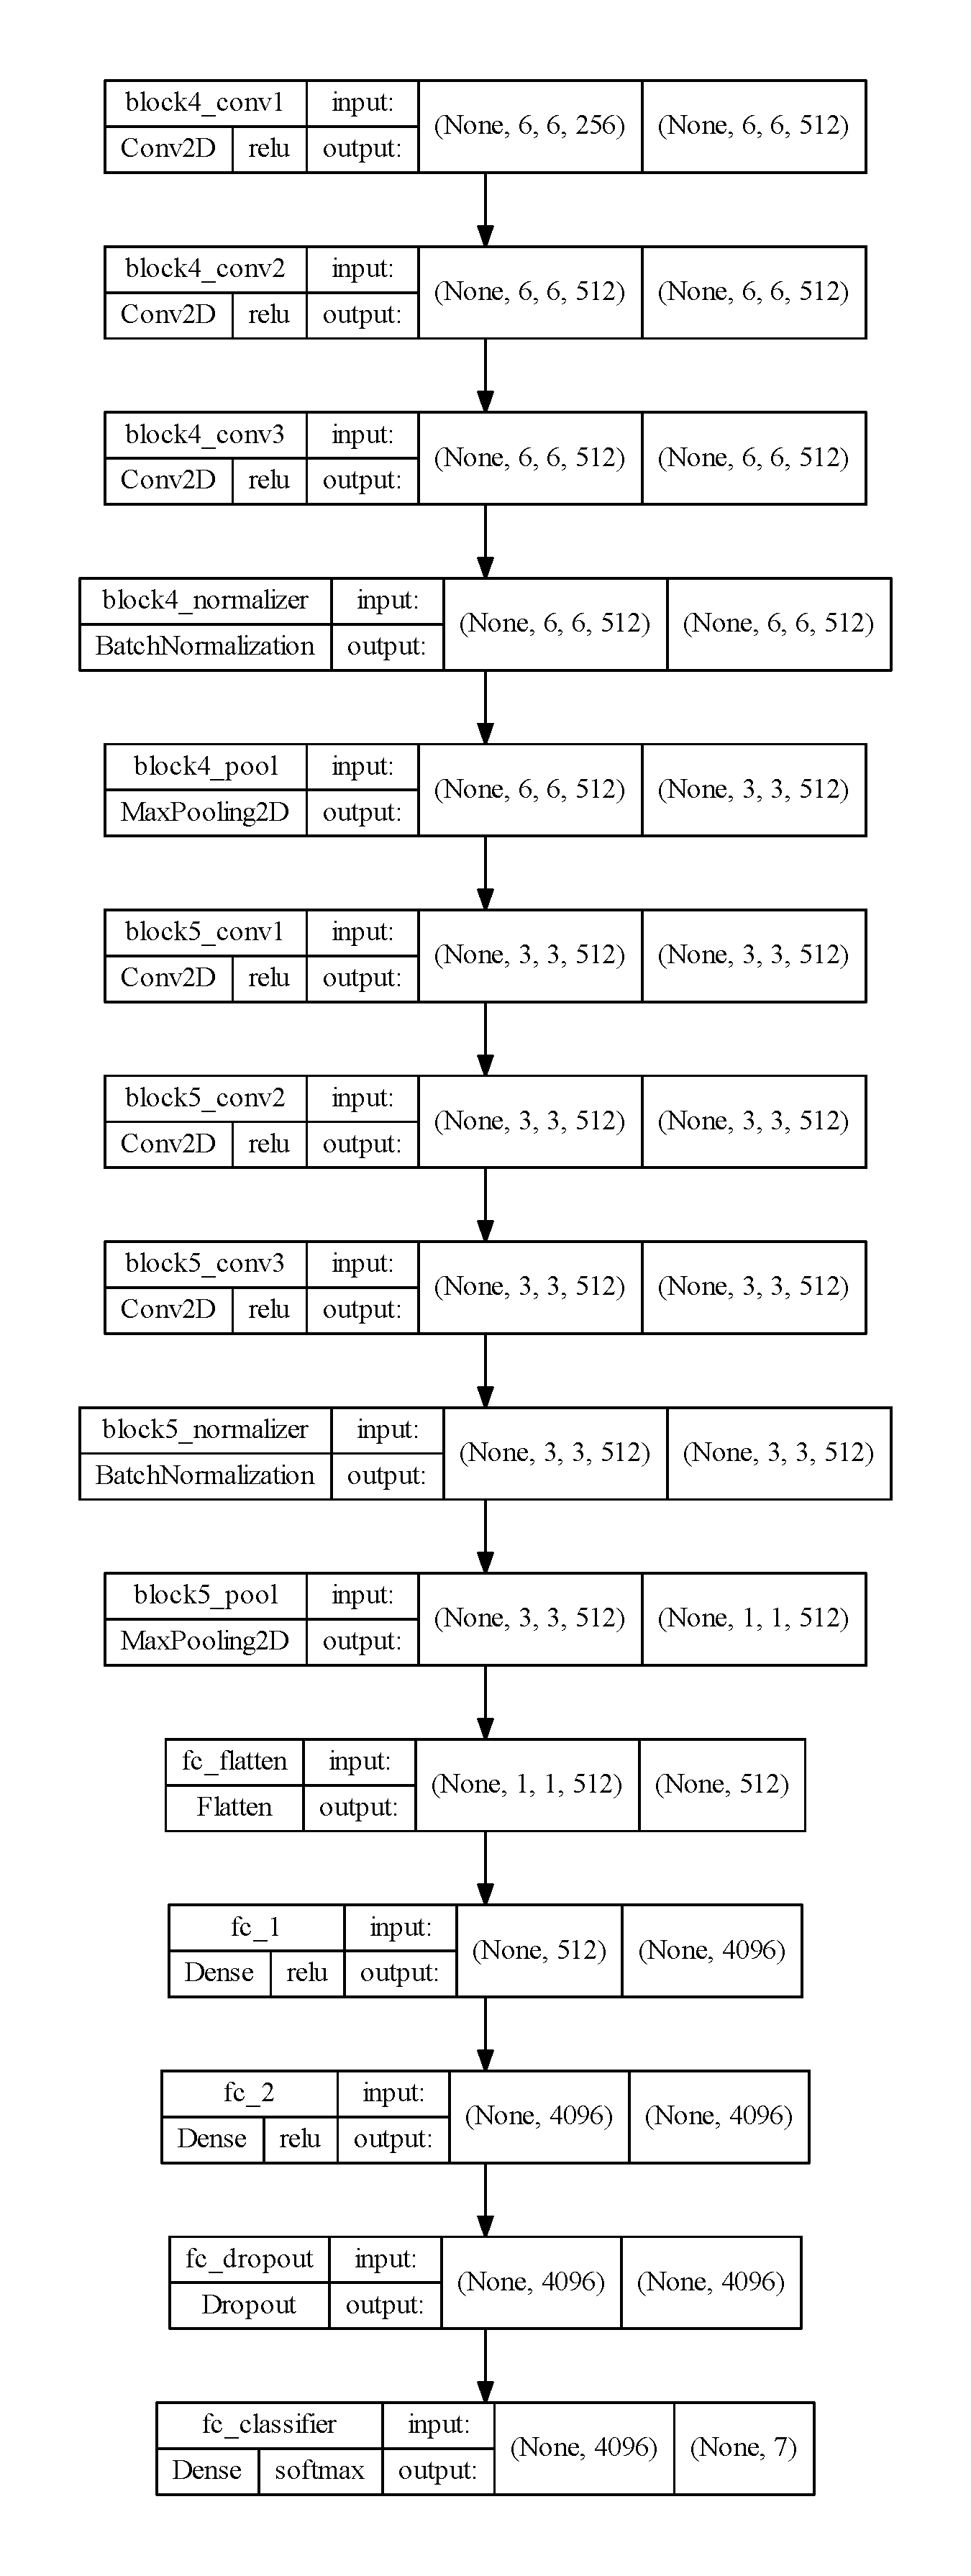
\includegraphics[height = 0.9\textheight]{written_report/pictures/model_2.pdf}
        \end{minipage}
        \caption{Model Architecture}
        \label{fig:model}
    \end{figure}
    
    \subsection{Model Training}
    \subsubsection{Training Specifications}
    Training a very deep CNN requires huge amount of GPU power, in which non of our group member could afford it. Thank to Google, they offer \href{https://research.google.com/colaboratory/}{Colab} which let us to train using their GPU for free.
    
    \subsubsection{Model Evaluation}
    \begin{figure}[H]
        \centering
        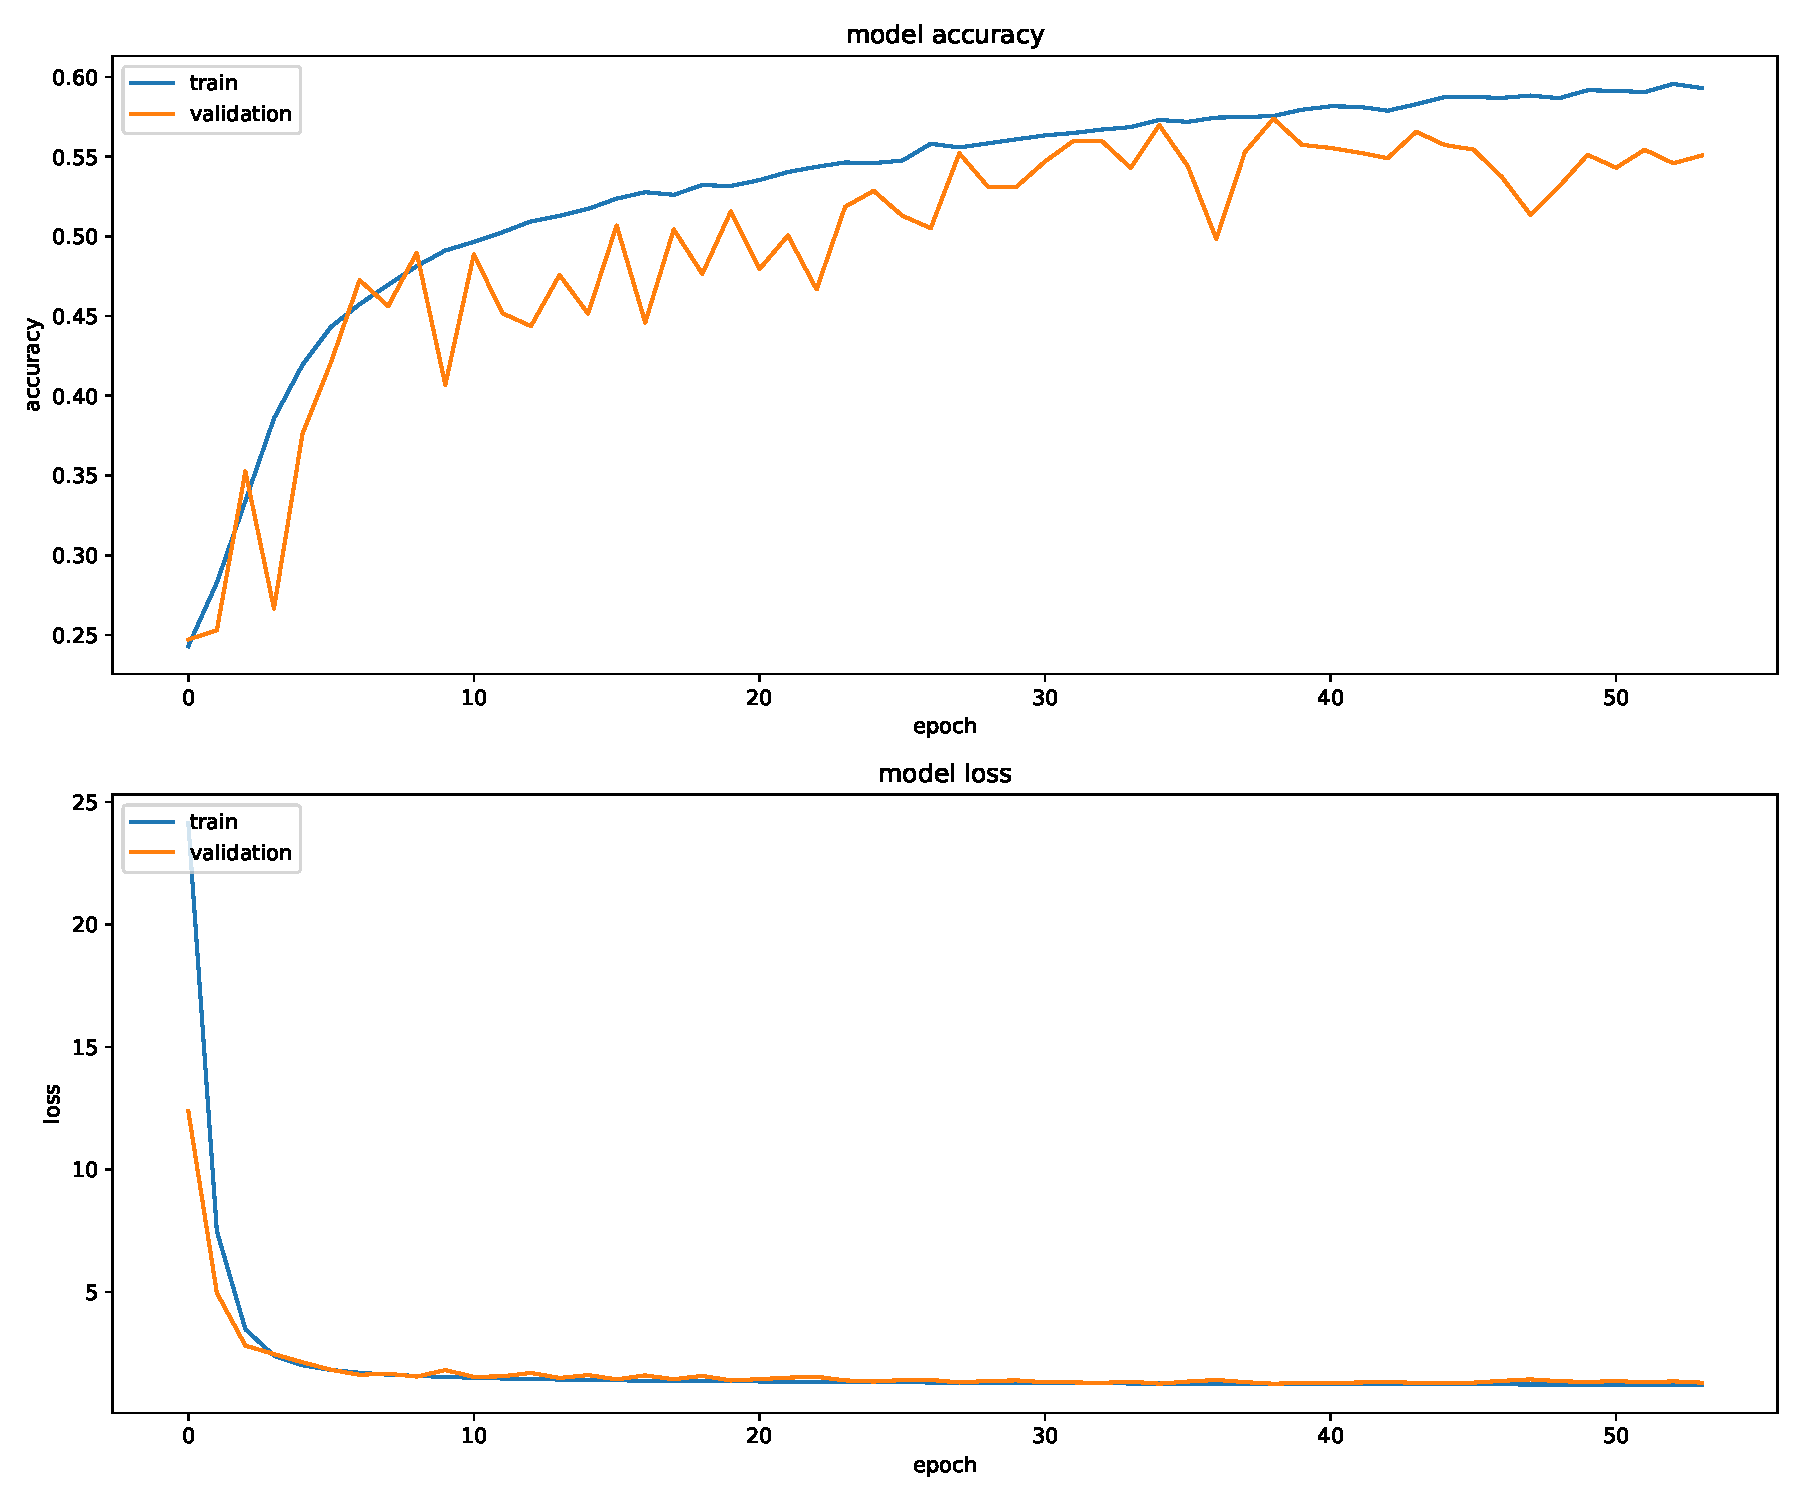
\includegraphics[width = 0.9\textwidth]{emotion_detection/plot/history.pdf}
        \caption{Loss and Accuracy}
        \label{fig:loss_acc}
    \end{figure}
    Early stopping was trigger after 54 epochs, the model eventually achieved valid accuracy at around 0.58.
    
    \subsection{Demonstration}
    
    \subsection{Conclusion}
    
    \newpage
    \section{Stock Price Forecasting}
    \textbf{This section is contributed by KWOK Ho Hin (SID: 1155126159), TSOI Tung Sing (SID: 1155127274) and LO Chak Kin Steven (SID: 1155125491).}
    
    \subsection{Introduction}
    
    
    \newpage
    % \thispagestyle{empty}
    % \pagenumbering{gobble} 
    \section{Bibliography}
    \bibliographystyle{unsrt}
    % \bibliographystyle{plain} % We choose the "plain" reference style
    \bibliography{refs} % Entries are in the refs.bib file
    
\end{document}